% !TeX root = ../../Book3.tex
% 纲要标题：### 4.4 子流形模型与曲率限制
% 纲要位置：几何学计划纲要.md，第 2251 行。
% 正文状态：初稿；尚未正式审核。

% 纲要内容开始
% 
% * 球面、乘积和管状模型
% * 超曲面的主曲率
% * 内在曲率相同而外在几何不同
% * 后续面积变分所需的公式
% 
% ---
% 
% 纲要内容结束

\section{子流形模型与曲率限制}
\label{g3:sec:0404}

相容方程把内在曲率、第二基本形式和法联络联系起来。具体计算时，可以从一个已知浸入求出这些量，再把它们代回方程；也可以先用曲率限制判断某种外在形状是否可能。球面、球面乘积和法向偏移提供了两种做法都能逐项核验的模型。最后，我们把平均曲率与体积密度的一阶变化联系起来。

\subsection{球面、乘积和管状模型}
\label{g3:subsec:0404:01}

在本小节的 Euclid 环境中，普通方向微分记为 \(\mathrm D\)。半径 \(a>0\) 的球面取外单位法向 \(\nu=f/a\)，则
\[
	\mathrm D_X\nu=\frac1a\mathrm df(X),\qquad
	A_\nu=-\frac1a I,\qquad
	B(X,Y)=-\frac1a g(X,Y)\nu,
	\qquad H=-\frac1a\nu.
\]
球面是全脐的，平均曲率向量指向球心。Gauss 方程却给出正截面曲率 \(a^{-2}\)，因为其中第二基本形式以两个因子的乘积出现。更换为内单位法向会反转 \(A_\nu\) 的符号，但不改变向量值的 \(B,H\) 或内在曲率。

\begin{example}\label{g3:exm:product-spheres-normal-data}
	设 \(p,q\ge1\)、\(a,b>0\)，考虑乘积浸入
	\[
		f:S^p(a)\times S^q(b)\longrightarrow
		\mathbb R^{p+1}\times\mathbb R^{q+1},\qquad f(x,y)=(x,y).
	\]
	记两个因子度量为 \(g_1,g_2\)，并在切丛另一因子上将它们补为零。法丛具有全局正交单位标架
	\[
		\nu_1=(x/a,0),\qquad \nu_2=(0,y/b).
	\]
	两者的环境导数均为切向量，故 \(\nabla^\perp\nu_1=\nabla^\perp\nu_2=0\)。直接求导得到
	\[
		B=-\frac{g_1}{a}\nu_1-\frac{g_2}{b}\nu_2,
		\qquad
		H=-\frac1{p+q}\left(\frac pa\nu_1+\frac qb\nu_2\right).
	\]
	两个形算子在乘积分解下同时对角化，彼此交换，法曲率为零。Gauss 方程对纯因子截面给出 \(a^{-2}\)、\(b^{-2}\)，对混合截面给出零；这与第三章的乘积曲率一致。当某个因子是一维时，只使用实际存在的二维截面。

	同一像还位于半径 \(L=\sqrt{a^2+b^2}\) 的球面中。相对于这个球面，单位法向可取
	\[
		\eta=\left(\frac{b}{aL}x,-\frac{a}{bL}y\right).
	\]
	它与位置向量正交，且长度为一。对两个因子的切向量求导，形算子的特征值分别是
	\[
		-\frac{b}{aL}\quad\text{（重数 \(p\)）},\qquad
		\frac{a}{bL}\quad\text{（重数 \(q\)）}.
	\]
	因此，这个乘积在球面中极小的充要条件为
	\[
		q a^2=p b^2,
		\qquad\text{即}\qquad
		a^2=\frac{p}{p+q}L^2,\quad b^2=\frac{q}{p+q}L^2.
	\]
	它在 Euclid 空间中的平均曲率向量始终非零。平均曲率依赖所选环境；切空间正交补改变后，第二基本形式所取的法向投影也随之改变。
\end{example}

沿各点的法方向移动，可以把子流形附近的空间组织成管状坐标。在 Euclid 空间中，这个构造只涉及向量加法；局部可逆性来自切向与法向的互补。

\begin{proposition}\label{g3:prop:euclidean-normal-tube}
	设 \(f:M^n\to\mathbb R^{n+r}\) 为光滑浸入，\(r\ge1\)，\(M\) 无边界。定义法丛上的映射
	\[
		\mathcal T:N_fM\longrightarrow\mathbb R^{n+r},
		\qquad \mathcal T(p,\xi)=f(p)+\xi.
	\]
	它在每个零向量 \((p,0)\) 的某个邻域上为微分同胚。若 \(M\) 紧且 \(f\) 为嵌入，则存在 \(\varepsilon>0\)，使 \(\mathcal T\) 将整个法圆盘丛 \(\{(p,\xi):|\xi|<\varepsilon\}\) 微分同胚地映到 \(f(M)\) 的一个开邻域。
\end{proposition}
\begin{proof}
	在局部法丛平凡化下，零截面处的切空间自然分成 \(\mathrm T_pM\oplus N_pf\)，且
	\[
		\mathrm d\mathcal T_{(p,0)}(X,\eta)=\mathrm df_p(X)+\eta.
	\]
	这是两个正交互补子空间到 \(\mathbb R^{n+r}\) 的线性同构。第一卷第11.3节的逆函数定理适用于同维光滑流形间的映射：一点处微分可逆便在该点附近有光滑逆。因此得到第一项结论。

	在紧情形，零截面紧，微分可逆性是开条件；有限覆盖给出共同的小半径，使 \(\mathcal T\) 在该法圆盘丛上处处为局部微分同胚。还要证明共同的小半径可以保证单射。若不能，则有两列不同点 \((p_j,\xi_j)\)、\((q_j,\eta_j)\)，满足 \(|\xi_j|,|\eta_j|\to0\) 且像相同。取子列使 \(p_j\to p\)、\(q_j\to q\)。像相同给出 \(f(p)=f(q)\)，嵌入的单射性使 \(p=q\)。在这个点的一个法丛平凡化中，两列点都收敛到 \((p,0)\)，与第一段得到的局部单射性矛盾。故足够小的半径可用。单射的局部微分同胚是到开像的微分同胚，且像包含 \(f(M)\)。
\end{proof}

上述开邻域称为一个\term[guanzhuanglinyu]{管状邻域}[tubular neighborhood]。仅有浸入时，不同分支的管状像可以相交；紧嵌入的证明同时使用了零截面的紧性与不同基点不能具有相同像。

\begin{proposition}\label{g3:prop:parallel-hypersurface}
	设 \(f:M^n\to\mathbb R^{n+1}\) 为带光滑单位法向 \(\nu\) 的光滑浸入，\(A=A_\nu\)。对常数 \(t\) 定义 \(f_t=f+t\nu\)。在 \(I-tA\) 可逆的开集上，\(f_t\) 仍为浸入，\(\nu\) 仍是其单位法向；相对于共同的参数流形，
	\begin{align}
		\mathrm df_t&=\mathrm df\circ(I-tA),
		&g_t(X,Y)&=g((I-tA)X,(I-tA)Y),\label{g3:eq:parallel-hypersurface-metric}\\
		A_t&=(I-tA)^{-1}A,
		&\mu_{g_t}&=|\det(I-tA)|\mu_g.\label{g3:eq:parallel-hypersurface-shape}
	\end{align}
\end{proposition}
\begin{proof}
	法丛是一维的，\(\langle\nu,\nu\rangle=1\) 使 \(\nabla^\perp\nu=0\)，故 \(\mathrm d\nu=-\mathrm df\circ A\)。对 \(f_t\) 求导便得到第一式。由于 \(\mathrm df\) 单射，\(\mathrm df_t\) 单射恰等价于 \(I-tA\) 可逆；其像仍是原切超平面，故 \(\nu\) 仍垂直于像。内积给出度量公式。对新浸入使用 Weingarten 公式，
	\[
		-\mathrm df(A X)=\mathrm d\nu(X)
		=-\mathrm df_t(A_tX)
		=-\mathrm df((I-tA)A_tX),
	\]
	从而得到 \(A_t\)。最后在正交基中取度量矩阵行列式及其正平方根，即得密度公式。
\end{proof}

对于外法向的半径 \(a\) 球面，\(I-tA=(1+t/a)I\)，所以外移后半径为 \(a+t\)，切向尺度乘以 \(1+t/a\)，密度乘以 \((1+t/a)^n\)。\cref{g3:fig:normal-offset}画出圆周的对应关系。

\begin{figure}[htbp]
	\centering
	% !TeX root = ../Book3.tex
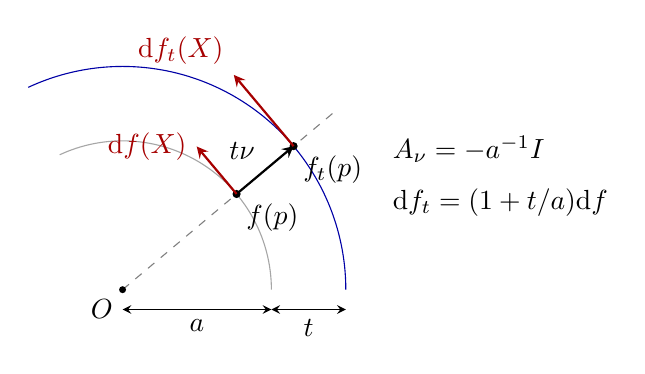
\begin{tikzpicture}[scale=1.05,>=stealth]
	\draw[gray!70] (0:1.8) arc[start angle=0,end angle=115,radius=1.8];
	\draw[blue!65!black] (0:2.7) arc[start angle=0,end angle=115,radius=2.7];
	\draw[gray,dashed] (0,0)--(40:3.35);
	\coordinate (P) at (40:1.8);
	\coordinate (Q) at (40:2.7);
	\fill (0,0) circle (1.2pt) node[below left]{\(O\)};
	\fill (P) circle (1.4pt) node[below right]{\(f(p)\)};
	\fill (Q) circle (1.4pt) node[below right]{\(f_t(p)\)};
	\draw[->,thick] (P)--(Q) node[midway,above left]{\(t\nu\)};
	\draw[->,thick,red!65!black] (P)--++(130:0.75) node[left]{\(\mathrm df(X)\)};
	\draw[->,thick,red!65!black] (Q)--++(130:1.125) node[above left]{\(\mathrm df_t(X)\)};
	\draw[<->] (0,-0.24)--(1.8,-0.24) node[midway,below]{\(a\)};
	\draw[<->] (1.8,-0.24)--(2.7,-0.24) node[midway,below]{\(t\)};
	\node[anchor=west] at (3.15,1.7){\(A_\nu=-a^{-1}I\)};
	\node[anchor=west] at (3.15,1.05){\(\mathrm df_t=(1+t/a)\mathrm df\)};
\end{tikzpicture}

	\caption[圆周的法向偏移]{圆周的外法向偏移。相同角参数的切向微分从内圆移到外圆后放大为原来的 \(1+t/a\) 倍。}
	\label{g3:fig:normal-offset}
\end{figure}

\subsection{超曲面的主曲率}
\label{g3:subsec:0404:02}

余维一时，每个法向值都由一个实数确定。选定单位法向 \(\nu\) 后，写 \(B(X,Y)=g(AX,Y)\nu\)。自伴算子 \(A\) 在每一点有正交单位特征基，其特征值 \(\kappa_1,\ldots,\kappa_n\) 称为该法向下的\term[zhuqulv]{主曲率}[principal curvatures]，相应特征方向称为\term[zhufangxiang]{主方向}[principal directions]。重特征值处未必能把单个主方向光滑选出，下面的逐点公式不需要这种选择。

\begin{proposition}\label{g3:prop:principal-curvature-contractions}
	设 \(f:(M^n,g)\to\bar M^{n+1}\) 是光滑等距浸入，\(n\ge2\)，环境截面曲率恒为 \(c\)。在一点选单位法向 \(\nu\) 及主方向正交单位基 \((e_i)\)，令 \(H_\nu=\langle H,\nu\rangle=n^{-1}\sum_i\kappa_i\)。则
	\begin{align}
		K(e_i,e_j)&=c+\kappa_i\kappa_j\quad(i\ne j),\label{g3:eq:principal-sectional-curvature}\\
		\operatorname{Ric}(e_i,e_j)
		&=\bigl((n-1)c+nH_\nu\kappa_i-\kappa_i^2\bigr)\delta_{ij},\label{g3:eq:principal-ricci-curvature}\\
		\operatorname{Scal}
		&=n(n-1)c+n^2H_\nu^2-|A|^2.\label{g3:eq:hypersurface-scalar-curvature}
	\end{align}
\end{proposition}
\begin{proof}
	Gauss 方程在这组基中成为
	\[
		R_{ijkl}
		=c(\delta_{ik}\delta_{jl}-\delta_{il}\delta_{jk})
		+\kappa_i\kappa_j(\delta_{ik}\delta_{jl}-\delta_{il}\delta_{jk}).
	\]
	取 \(k=i,l=j\) 得到截面公式。固定 \(i\)，把它对 \(j\ne i\) 相加，得到
	\[
		\operatorname{Ric}(e_i,e_i)
		=(n-1)c+\kappa_i\Bigl(\sum_j\kappa_j-\kappa_i\Bigr).
	\]
	非对角分量由同一四阶公式为零。再对 \(i\) 求和，使用 \(|A|^2=\sum_i\kappa_i^2\)，即得标量曲率式。
\end{proof}

这些公式也给出外在形状的限制。例如 Euclid 超曲面若在一点平坦，则 \(\kappa_i\kappa_j=0\) 对所有 \(i\ne j\) 成立，故该点形算子的秩至多为一。若每个截面曲率都严格为正，则任意两个主曲率的乘积均为正，所有主曲率同号。另一方面，全脐点的 \(A=H_\nu I\) 使所有截面曲率等于 \(c+H_\nu^2\)。

\ProseParagraphBreak

法向偏移的主曲率可由式\eqref{g3:eq:parallel-hypersurface-shape}逐个读取：
\[
	\kappa_i(t)=\frac{\kappa_i}{1-t\kappa_i}.
\]
当某个 \(1-t\kappa_i\) 为零时，相应切向方向被 \(\mathrm df_t\) 压为零，偏移参数化失去浸入性。这是一个局部微分条件。即使这些因子都非零，不同基点的法线仍可能在远处相交，因此共同管状半径还需要控制整体单射性。

\subsection{内在曲率相同而外在几何不同}
\label{g3:subsec:0404:03}

内在度量记录沿子流形测量的长度，第二基本形式则记录切空间在环境中的转动。同一度量可以对应不同的第二基本形式；局部基本定理的唯一性因而需要完整的相容数据。

\begin{example}\label{g3:exm:plane-cylinder-isometry}
	在一个平面开矩形 \(U\subset\mathbb R^2\) 上，考虑
	\[
		f_0(u,v)=(u,v,0),\qquad
		f_a(u,v)=\bigl(a\cos(u/a),a\sin(u/a),v\bigr),\quad a>0.
	\]
	两者的诱导度量都是 \(\mathrm du^2+\mathrm dv^2\)，所以具有相同的内在距离局部结构和零 Gauss 曲率。对圆柱取外法向
	\[
		\nu(u,v)=\bigl(\cos(u/a),\sin(u/a),0\bigr),
	\]
	则 \(A_\nu\partial_u=-a^{-1}\partial_u\)、\(A_\nu\partial_v=0\)，而平面上 \(B=0\)。故两者不可能在任何开集上由一个 Euclid 刚性运动联系：环境等距保持第二基本形式，尤其保持其范数。这里一个范数为零，另一个为 \(a^{-1}\)。

	若允许 \(u\) 遍历整个实轴，\(f_a(u+2\pi a,v)=f_a(u,v)\)。因此这个局部等距参数化在整个平面上不单射；把参数域限制到适当的小矩形后，才得到到一块圆柱面的等距微分同胚。
\end{example}

上述区别在高余维中还包括法联络。即使给定相同的 \(g\) 和对称型的分量，换法标架时也必须同时按同一个丛等距变换法联络与 \(B\)。三组相容方程正是对这套几何数据的条件；只比较一张矩阵或只比较内在曲率，不能使用基本定理的唯一性结论。

\subsection{后续面积变分所需的公式}
\label{g3:subsec:0404:04}

当浸入随参数移动时，切向速度主要改变参数点的分布，法向速度才直接与平均曲率配对。先计算诱导度量及其体积密度的导数，便能在任意维数、任意余维得到面积的一阶公式。这里“面积”指 \(n\) 维诱导体积；对非单射浸入按参数流形积分，保留重数。

\begin{theorem}[面积的一阶变分]\label{g3:thm:first-variation-submanifold-area}
	设 \(F:(-\varepsilon,\varepsilon)\times M^n\to(\bar M,\bar g)\) 光滑，每个 \(f_t=F(t,\cdot)\) 都是浸入，\(n\ge1\)。记 \(g_t=f_t^*\bar g\)、\(g=g_0\)，并将初速度分解为 \(V=\partial_tF|_0=\mathrm df_0(W)+V^\perp\)。则
	\begin{align}
		\dot g_0(X,Y)
		&=g(\nabla_XW,Y)+g(X,\nabla_YW)
		-2\langle B(X,Y),V^\perp\rangle,\label{g3:eq:variation-induced-metric}\\
		\left.\frac{\mathrm d}{\mathrm dt}\right|_0\mu_{g_t}
		&=\bigl(\operatorname{div}_gW-n\langle H,V^\perp\rangle\bigr)\mu_g.\label{g3:eq:variation-induced-density}
	\end{align}
	若 \(\Omega\subset M\) 是具有光滑边界的紧区域，\(\eta\) 是 \(\partial\Omega\) 在 \(M\) 内的外单位法向，则
	\begin{equation}\label{g3:eq:first-variation-area-integral}
		\left.\frac{\mathrm d}{\mathrm dt}\right|_0\operatorname{Vol}_{g_t}(\Omega)
		=\int_{\partial\Omega}g(W,\eta)\mu_{\partial g}
		-n\int_\Omega\langle H,V^\perp\rangle\mu_g.
	\end{equation}
\end{theorem}
\begin{proof}
	把 \(X,Y\) 延拓成与时间无关的参数向量场。环境联络度量相容且无挠，因而沿二参数坐标面有 \(\bar\nabla_t\mathrm df_t(X)=\bar\nabla_X\partial_tF\)。逐项求导得到
	\[
		\dot g_0(X,Y)
		=\langle\bar\nabla_XV,\mathrm df_0(Y)\rangle
		+\langle\mathrm df_0(X),\bar\nabla_YV\rangle.
	\]
	代入 \(V=\mathrm df_0(W)+V^\perp\)，用 Gauss 分解和 Weingarten 公式提取切向分量，便得度量变化式。

	在任一固定坐标中，密度系数为 \(\sqrt{\det g_t}\)。可逆矩阵的行列式求导给出
	\[
		\left.\frac{\mathrm d}{\mathrm dt}\right|_0\sqrt{\det g_t}
		=\frac12\operatorname{tr}_g(\dot g_0)\sqrt{\det g}.
	\]
	在一点取正交单位基求迹，前两项各贡献 \(\operatorname{div}_gW\)，最后一项贡献 \(-2n\langle H,V^\perp\rangle\)。这证明密度公式。紧区域上可在积分号下求导，再对 \(W\) 使用\cref{g3:thm:divergence-theorem}，得到边界通量。密度与该散度定理均不要求 \(M\) 可定向。
\end{proof}

\begin{corollary}\label{g3:cor:minimal-area-stationarity}
	设 \(f:M^n\to\bar M\) 为光滑浸入，\(n\ge1\)，\(M\) 无边界。则 \(H=0\) 当且仅当对于任意具有光滑边界的紧区域 \(\Omega\subset M\)，以及任意满足 \(\operatorname{supp}V\subset\operatorname{int}\Omega\) 的上述光滑变分，都有 \(\left.\frac{\mathrm d}{\mathrm dt}\right|_0\operatorname{Vol}_{g_t}(\Omega)=0\)。
\end{corollary}
\begin{proof}
	若 \(H=0\)，在包含初速度支集的紧区域上应用式\eqref{g3:eq:first-variation-area-integral}，边界项和内部项都为零。反过来，若某点 \(H\ne0\)，在其附近选一个非负光滑截断函数 \(\chi\)，支集紧含于一个坐标片，且在该点附近为正。取法向初速度 \(V=\chi H\)。它可以由变分
	\[
		f_t(p)=\exp^{\bar g}_{f(p)}(tV(p))
	\]
	实现：支集紧使共同的小时间可用，指数映射的联合光滑性见\cref{g3:prop:exponential-local}；浸入性是开条件，在这个紧支集上缩小时间便仍成立，支集外则保持原映射。此时一阶变分为 \(-n\int\chi|H|^2\mu_g<0\)，与驻定性矛盾。因此 \(H\) 必处处为零。
\end{proof}

这一结论说明“极小”的一阶意义是面积驻定。是否在所有邻近变分下取得局部最小值，还需要二阶变化的信息。球面外移的检验则直接固定本章符号：若 \(V=\nu\)、\(H=-\nu/a\)，密度导数为 \(n\mu_g/a>0\)，与半径增大一致。

\begin{proposition}\label{g3:prop:immersion-position-laplacian}
	设 \(f:(M^n,g)\to\mathbb R^{n+r}\) 为光滑等距浸入，\(n\ge1\)，对位置向量的各坐标分别使用 \(\Delta_g=-\operatorname{div}_g\operatorname{grad}_g\)。则
	\begin{equation}\label{g3:eq:position-laplacian}
		\Delta_g f=-nH,\qquad
		\Delta_g|f|^2=-2n-2n\langle f,H\rangle.
	\end{equation}
	若像位于 \(S^{n+r-1}(a)\)，以 \(H^S\) 表示相对于球面的平均曲率向量，则
	\begin{equation}\label{g3:eq:spherical-minimal-eigenmap}
		H^{\mathbb R}=H^S-\frac f{a^2},\qquad
		H^S=0\ \Longleftrightarrow\ \Delta_g f=\frac n{a^2}f.
	\end{equation}
\end{proposition}
\begin{proof}
	对任一坐标函数 \(f^\alpha\)，Hessian 的定义给出
	\[
		H_{f^\alpha}(X,Y)
		=\bigl(\mathrm D_X\mathrm df(Y)-\mathrm df(\nabla_XY)\bigr)^\alpha
		=B(X,Y)^\alpha.
	\]
	取负迹即得 \(\Delta_g f=-nH\)。由乘积法则，
	\[
		\Delta_g|f|^2=2\langle f,\Delta_g f\rangle-2|\mathrm df|^2.
	\]
	等距浸入使 \(|\mathrm df|^2=n\)，故得第二式。若像在半径 \(a\) 的球面内，先将环境导数投影到球面的切空间，再投影到 \(M\) 的切空间；球面自身的第二基本形式为 \(-g f/a^2\)。于是
	\[
		B^{\mathbb R}(X,Y)=B^S(X,Y)-\frac{g(X,Y)}{a^2}f.
	\]
	取平均迹得到两个平均曲率的关系，再代入位置向量的 Laplace 公式，便得最后的等价式。
\end{proof}

\begin{corollary}\label{g3:cor:no-compact-euclidean-minimal}
	正维紧无边界光滑流形不存在到 Euclid 空间的极小浸入。
\end{corollary}
\begin{proof}
	若有这样的浸入，以诱导度量计算，由 \(H=0\) 及式\eqref{g3:eq:position-laplacian}，有 \(\Delta_g|f|^2=-2n\)。在 \(M\) 上积分，散度定理使左边为零，右边却是 \(-2n\operatorname{Vol}_g(M)<0\)，矛盾。
\end{proof}

球面中的极小乘积没有这一矛盾：其 Euclid 平均曲率为 \(-f/a^2\)，在位置向量公式中恰好抵消常数项。这样，局部的切法分解、相容方程及整体积分在同一个模型上相互核对。
